\section{ChargE3Net}


\begin{frame}{ChargE3Net Architecture Overview}
    \begin{itemize}
        \item Based on the E3NN backbone.
        \item Construct two k-d trees to partition the atoms and probes.
        \item Two types of convolutions:
        \begin{itemize}
            \item Conv$_{\text{atom}}$: Bidirectional between atoms
            \begin{equation*}
                \text{Conv}_{\text{atom}}^n(\mathbf{r}_i, X_i^n) = 
                W_1^n (\sum_{j \in \partial(i)}W_2^nX_j^n \otimes R(r_{ij})Y(\mathbf{r}_{ij}))
                + W_3^n X_i^{n}.
            \end{equation*}
            \item Conv$_{\text{probe}}$: From atoms to probes, only contains neighboring
            atoms, no probe-probe interactions.
        \end{itemize}
        \item Training objective:
        \begin{align*}
            \mathcal{L} &= \frac{\sum_{\mathbf{r} \in G} |\rho(\mathbf{r}) - \hat{\rho}(\mathbf{r})|}{
                \sum_{\mathbf{r} \in G} |\rho(\mathbf{r})|}
        \end{align*}
    \end{itemize}
\end{frame}


\begin{frame}{Model performance}
    \begin{itemize}
        \item Vertices:
        \begin{itemize}
            \item Atoms: One-hot encoding of atomic number; reps = Nx0o.
            \item Probe points: Initialized as zero scalar; reps = 1x0o.
        \end{itemize}
        \item Edges:
        \begin{itemize}
            \item Atom-atom: Unidirectional, cutoff 4Å
            \item Atom-probe: Directed from atoms to probes
        \end{itemize}
        \item Periodic boundary conditions supported
    \end{itemize}
    \begin{figure}
        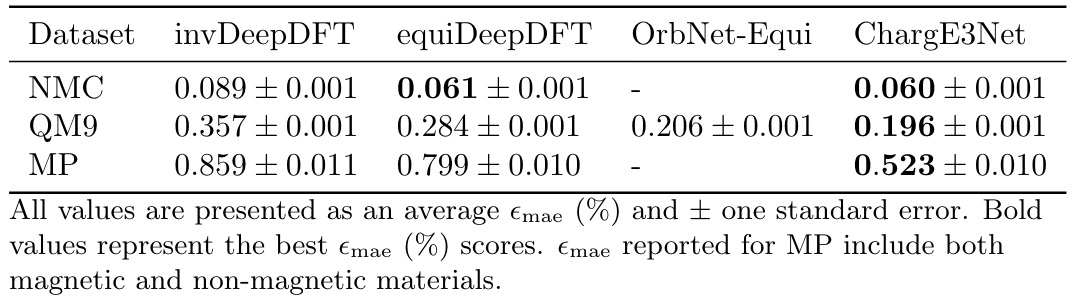
\includegraphics[width=\textwidth]{figures/charge3net_1.jpg}
    \end{figure}
\end{frame}


\begin{frame}{Performance}
    \begin{itemize}
        \item Accelerate DFT calculations: MP materials: 26.7\% reduction;
        GNoME materials: 28.6\% reduction.
        \item Non-self-consistent property prediction:
        \begin{itemize}
            \item 40\% of materials: energy errors < 1 meV/atom
            \item 70\% of materials: forces < 0.03 eV/Å
            \item 76\% of materials: band gaps within chemical accuracy
        \end{itemize}
        \item Linear scaling O(N) with system size.
    \end{itemize}
    \begin{figure}
            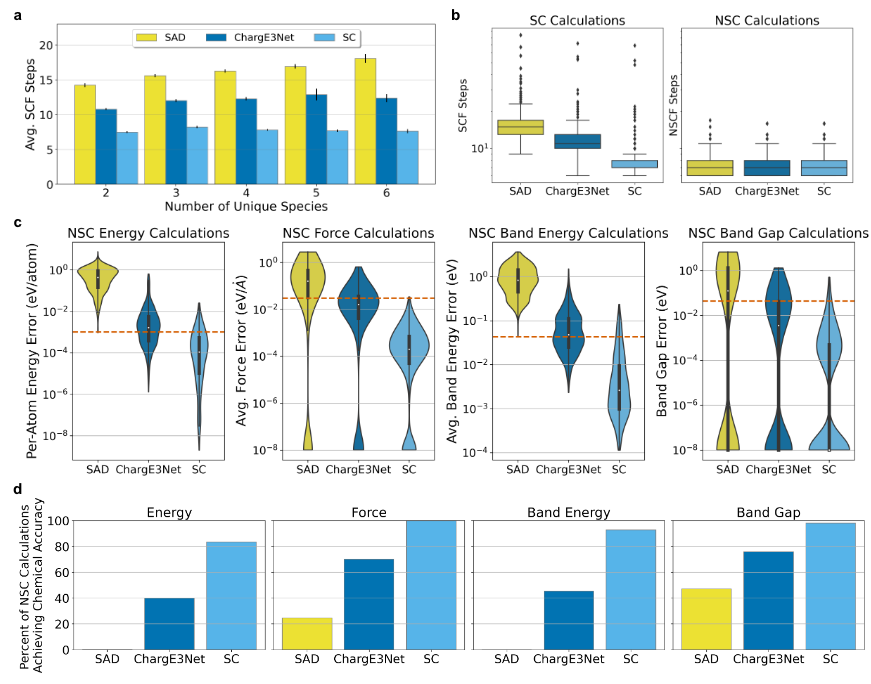
\includegraphics[width=.42\textwidth]{figures/charge3net_2.jpg}
            \caption{}
    \end{figure}
\end{frame}


\begin{frame}{Effect of higher-order features}
    \begin{itemize}
        \item The total dimension of features is N.
        \item With highest order $L$, The dimension of each order is $N/(L + 1)$.
        \item The channel of order $l$ is $N / (L + 1) / (2l + 1)$.
    \end{itemize}
    \begin{figure}
            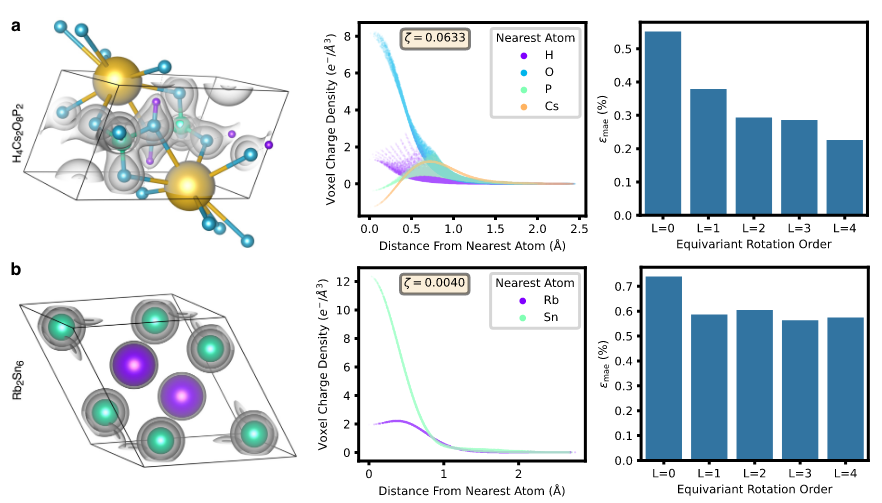
\includegraphics[width=.8\textwidth]{figures/charge3net_3.jpg}
            \caption{}
    \end{figure}
\end{frame}


\begin{frame}{Angular Variance Analysis}
    \begin{itemize}
        \item Performance improvement:
        \begin{itemize}
            \item 44.6\% median improvement for materials with non-metals/metalloids
            \item 23.0\% median improvement for materials with only metals
        \end{itemize}
        \item Metric $\zeta$ for angular variance:
        \[
        \zeta(G) = 1 - \frac{\sum_{\vec{g}_k \in G} |\nabla\rho(\vec{g}_k) \cdot \hat{r}_{ki}|}{\sum_{\vec{g}_k \in G} ||\nabla\rho(\vec{g}_k)||}
        \]
        \item High angular variance materials, e.g. Cs(H2PO4)
        \begin{itemize}
            \item Strong covalent bonding
            \item Significant L=4 improvement
        \end{itemize}
        \item Low angular variance materials, e.g. Rb2Sn6:
        \begin{itemize}
            \item Primarily ionic interactions
            \item Similar L=0 and L=4 performance
        \end{itemize}
    \end{itemize}
\end{frame} 